%\documentclass[numbers=noenddot, 12pt, a4paper, oneside]{scrbook}%
\documentclass[12pt, a4paper]{report}
\usepackage{blindtext}
\usepackage{fullpage}
\usepackage[utf8]{inputenc}
\usepackage{float}
\usepackage{hyperref}
\usepackage{hyperref}
\usepackage{tabularx}
\usepackage{graphicx}
\def\Plus{\texttt{+}}
\usepackage{listings}
\usepackage{xcolor}

\begin{document}

\begin{titlepage}
	\centering
	\vspace{1cm}
	\vspace{1cm}

	{\scshape\Large Game Design Document\par}
	\vspace{0.1cm}
	\begin{figure}[H]
		\centering
		\includegraphics[width=0.5\textwidth]{images/Logo}
	\end{figure}
	\vspace{1cm}
	\vspace{3cm}
	{\Large\itshape by\par}
	{\Large\itshape Gianluigi Oliva\par}
	{\Large\itshape Filippo Ghinelli, Leonardo Febbo, Lucia Ferrari\par}
	\vspace{1.5cm}
	\vfill
	


	\vfill

	% Bottom of the page
	{\large \today\par}
\end{titlepage}

\newpage
\tableofcontents
\newpage

\chapter{Overview and General Idea}
\section*{Introduction}
A terrible malware infected Tommy’s computer and he cannot use it anymore. When everything seemed to be lost, here it comes: a help from a little hero…a Bit. Our hero will have to travel to the heart of the pc: the kernel, fixing all the bugs caused by the malware and destroy it. Start with the high-level applications, such as a browser, and go on to the operative system to solve various problems. Free the imprisoned programs and ask them to help you during your adventure.\\

This is a 2D puzzle game with cooperative and platforming elements designed for PC. The visual style is simple and cartoony.

\section*{Description}
The player must solve puzzles to reach the exit. The world is arranged in an upside-down pyramid structure, divided in several layers: from the top to the bottom there is the Software Application Layer, then the Operating System Layer and lastly the System Kernel Layer. Our hero’s story is set in the Software Application Level, where he will travel through partitions and meet his allies. Inside the partitions, Bitty must progress through different levels.

In addition to the protagonist, the player will be able to control other programs released during the game and exploit their different skills. In the levels there are also enemies and sensors that will immediately trigger an alarm, so it is necessary not to be spotted. The player can only control one character at a time, so he should change control when all the characters are safe. Therefore, in this game, platforming, puzzles and co-op elements are combined.

To complete each level it is necessary to collect the key to open the exit and then reach the door with \textit{all} characters that are available.

\section*{Audience and Marketing}
The game is designed to appeal to all ages, starting from the cartoony and friendly graphics. The individual puzzles have a degree of complexity such that they are entertaining for casual and hardcore gamers alike.\\
The principal competitors of this game are games like “Thomas Was Alone” where there is a strong cooperation factor between the characters, or “Fez” for his puzzle component.

\section*{Genre(s)}
Platformer, Stealth, Puzzle
\section*{Platform(s)}
Windows 10, MacOS
\section*{Number of Players}
Single Player

\chapter{Principal Game Mechanics and Gameplay}
The principal mechanic of this game is the cooperation between the characters, the different level elements and avoiding Virus enemies, as well as using the characters’ skills to create combinations and different interactions within the level.

\section*{Basic skills}
These are the basic skills and mechanics for all the characters that the player can control:
\begin{itemize}
	\item \textbf{Walk}: The basic movement action of the characters. It gives a sense of mass and gravity, without slowing down movement.
	\item \textbf{Jump}: The character is able to jump but it can be possible to change direction while in air, and gravity is treated like in the real world. Like for the action of walking, a sense of mass and weight is present. 
	\item \textbf{Interacting} with levers, buttons and boxes: The character is able to interact with predefined machineries and levers to make something happen within a level.
\end{itemize}

Level failure can be caused by:
\begin{itemize}
	\item being detected from a "Resident",
	\item going through a laser sensor,
	\item being hitted from an enemy,
	\item touching an enemy,
	\item falling in traps.
\end{itemize}
This is valid for all the characters.



\section*{Character’s skills}
Each character has a unique skill which can be used in different ways to solve a puzzle:
\begin{itemize}
	\item \textbf{Bitty}: the protagonist and the starting character of the game, he can collect one bit at a time and fire it in the direction he’s facing. The bits can be used to get rid of Spywares and to activate switches.
	\item \textbf{Shieldy}: a program who can stun Viruses from behind. This ability can be turned on or off and covers a circular area around the 				character. A Virus will remain stunned as long as it remains within the area of effect, otherwise it will come to its senses after 5 seconds.
	\item \textbf{Zippy}:  a program who can shrink himself horizontally or vertically, gaining respectively height or width. He can also shrink allies if they are near him, but only vertically.
	\item \textbf{Gimpy}: a program who can camouflage herself to avoid being seen from enemies but he is still tangible.
\end{itemize}

\section*{Viruses' skills}
There are different Virus enemies in the game, each one representing a different kind of computer virus. Each enemy has a particular feature and behaviour:
\begin{itemize}
	\item \textbf{Resident}: The Resident is a sentinel with a very wide field of vision. If he identifies the player he launches an alarm that leads to the game 		over. This enemy stays still, it is dangerous only if the player touches it.
	\item \textbf{Trojan}: The Trojan is an enemy which protects a specific area in a level. If he spots the player,it will charge towards him at high speed. If it misses, it will turn back to its original position.
	\item \textbf{Spyware}: The Spyware is an enemy hanging from the ceiling that moves from top to bottom. It is harmless until the player walks below it: it will then drop down incredibly fast and most certainly catch the player.
	\item \textbf{Worm}: The Worm is a very large and heavy enemy, almost impossible to move or neutralize. He blocks the way, preventing progress through the level.
	\item \textbf{Infector}: The Infector is a virus that propagates simply by touching the areas of a level, making them deadly to the touch.
	\item \textbf{Keylogger}: An enemy which mimics exactly the movements of a character.
\end{itemize}




\section*{Camera}
%Since the game is based on puzzle resolution, the player must always have a complete view of the map, so a static camera is used which always shows the entire level and it's positioned at a fixed distance.\\
%Each time the player finishes a level the camera will show the next level, after a small cutscene. The camera will not be static only during the tutorial phase, which consists of a sliding level in which the player will experience all the basic mechanics.

Since the game is based on the resolution of the puzzles, the camera will show a large portion of the environment in a way to have on the screen most of the elements needed to solve the puzzles. The camera is centered on the active character and will move smoothly if the character is switched.

\section*{Hazards}
Viruses are not the only thing that the player must avoid.
\begin{itemize}
	\item \textbf{Laser}: Lasers kill anyone who touches them. Some lasers are stationary, while others can rotate either by default or by interacting with a 			terminal, but they can't be turned off. These are generated by an emitter positioned around the level. These lasers have no effect on anything other than a character, but they can be blocked by elements of a level like blocks.
	\item \textbf{Spikes}: Spikes are generally positioned in pits and kill anyone who falls on them. However it is possible to place objects over them in order to jump past them.
\end{itemize}

\section*{Interactables}
The principal mechanisms in a level are:
\begin{itemize}
	\item \textbf{Buttons}: Some can be pressed once to activate something, while others need a constant pressure to stay activated. The buttons can be activated by anything tangible, like characters or objects.
	\item \textbf{Blocks}: They have weight and they can be pushed around the level to climb to higher places or keep buttons presed.
	\item \textbf{Moving Platform or Elevators}: they can carry everything that is on them. Some move on their own from the start while others must be activated with the press of a button or a switch.
	\item \textbf{Barriers/Gates}: They are used to make inaccessible some areas. By activating a button they can be deactivated or opened.
	\item \textbf{Terminal}: They have an “on” state and an “off” state. For example, the player can change the direction of a laser by using a terminal.
\end{itemize}

\section*{Control System}
The in-game movement, like most of the puzzles, is physics-based. The control system also takes care of the changing of the controlled character ensuring that at any time the player can use only one character at a time. To make the player understand which character he is controlling in a precise moment, the system activates an UI indicator.



\chapter{Story and World}
The entire game is set inside a PC of a young boy, Tommy. Tommy’s PC got infected by a terrible virus which has made the pc unusable and he doesn’t know how to fix this problem. Tommy is unaware that a single brave bit is going to help him, so he is thinking of formatting the disk. The protagonist has little time to destroy the Viruses but alone he is not enough to stop such a catastrophe, so he needs to find other programs to help him in saving his world. However, they have been captured by the Viruses and Bitty must find a way to free them first.\\
The world is an upside-down pyramid structure, much like Dante’s Inferno, starting from the Software Application Layer, going through the Operating System Layer and reaching the core, the System Kernel Layer. These layers or zones are divided into levels with puzzles. When a level begins, a small cutscene will advance the plot.

\section*{Characters}
Each character has an own personality:
\begin{itemize}
\item \textbf{Bitty}: A small and very determined bit. Since he is a character of few words, he prefers to act instead to speak.
\item \textbf{Shieldy}: A program with a very strong sense of justice. He protects the others by blocking all kind of viruses with his shield.
\item \textbf{Zippy}: A timid and introverted program. He handles most problems by shrinking down and finding a way around them.
\item \textbf{Gimpy}: Who said the programs are all male? She is a program of a certain age, but thanks to her great touch-up skills she seems to be younger. Sparkling and dynamic she always keeps the mood high with its photomontages.
\end{itemize}

\chapter{Art Overview}
The visual style for the environment is simple and linear and allows the player to imagine being inside a computer.
The playable characters are pill-shaped, with stubby limbs and cutesy button-like eyes. Bitty, Zippy and Gimpy have marks and features on their bodies which evoke their abilities. Shieldy and Gimpy carry their signature items with them, as a reminder to the player of what they can do.\\
The Viruses' bodies are more menacing, starting from their angry-looking eyes, sharper edges and more complex shapes.\\

\section*{Sketch and Characters Design}
\begin{figure}[H]
	\centering
	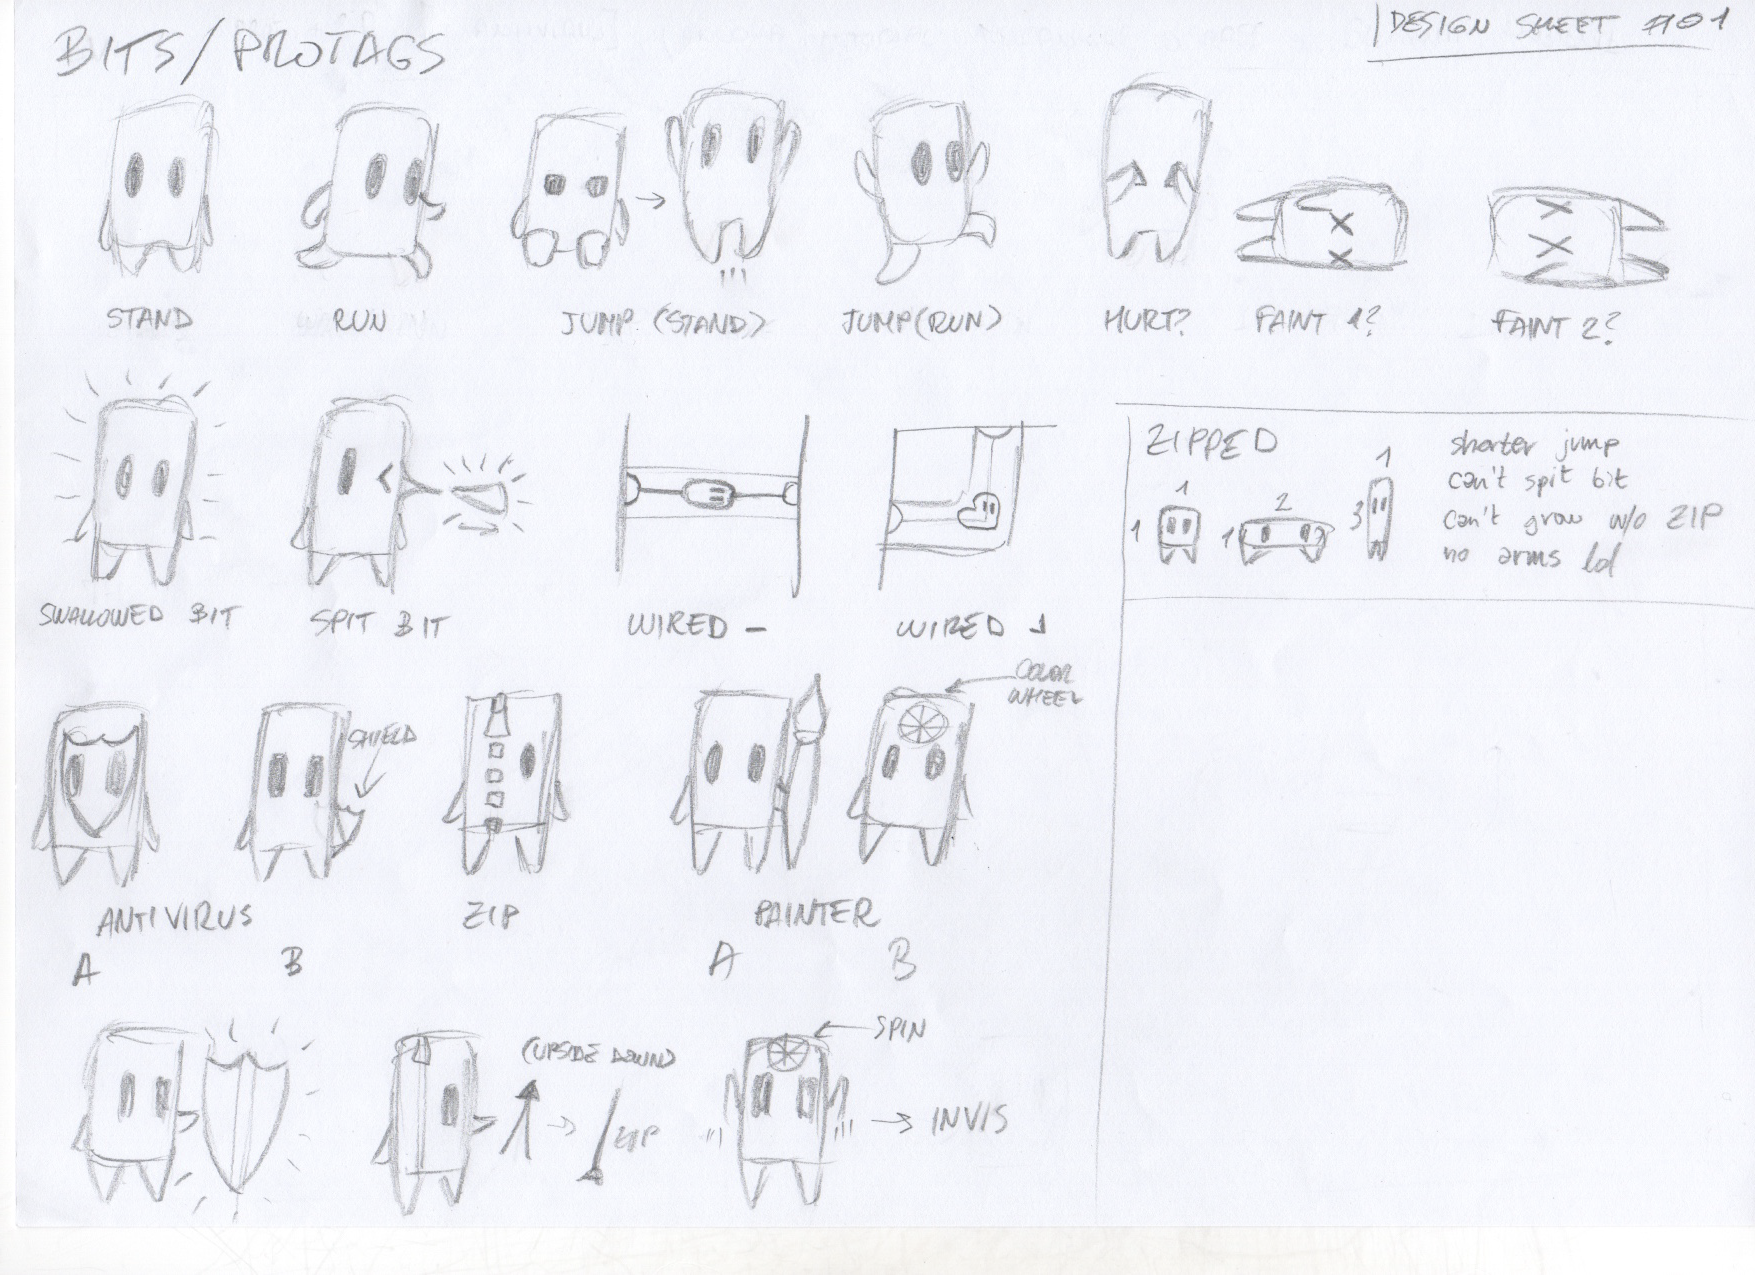
\includegraphics[width=0.5\textwidth]{images/Characters}
\end{figure}
	\begin{figure}[H]
	\centering
	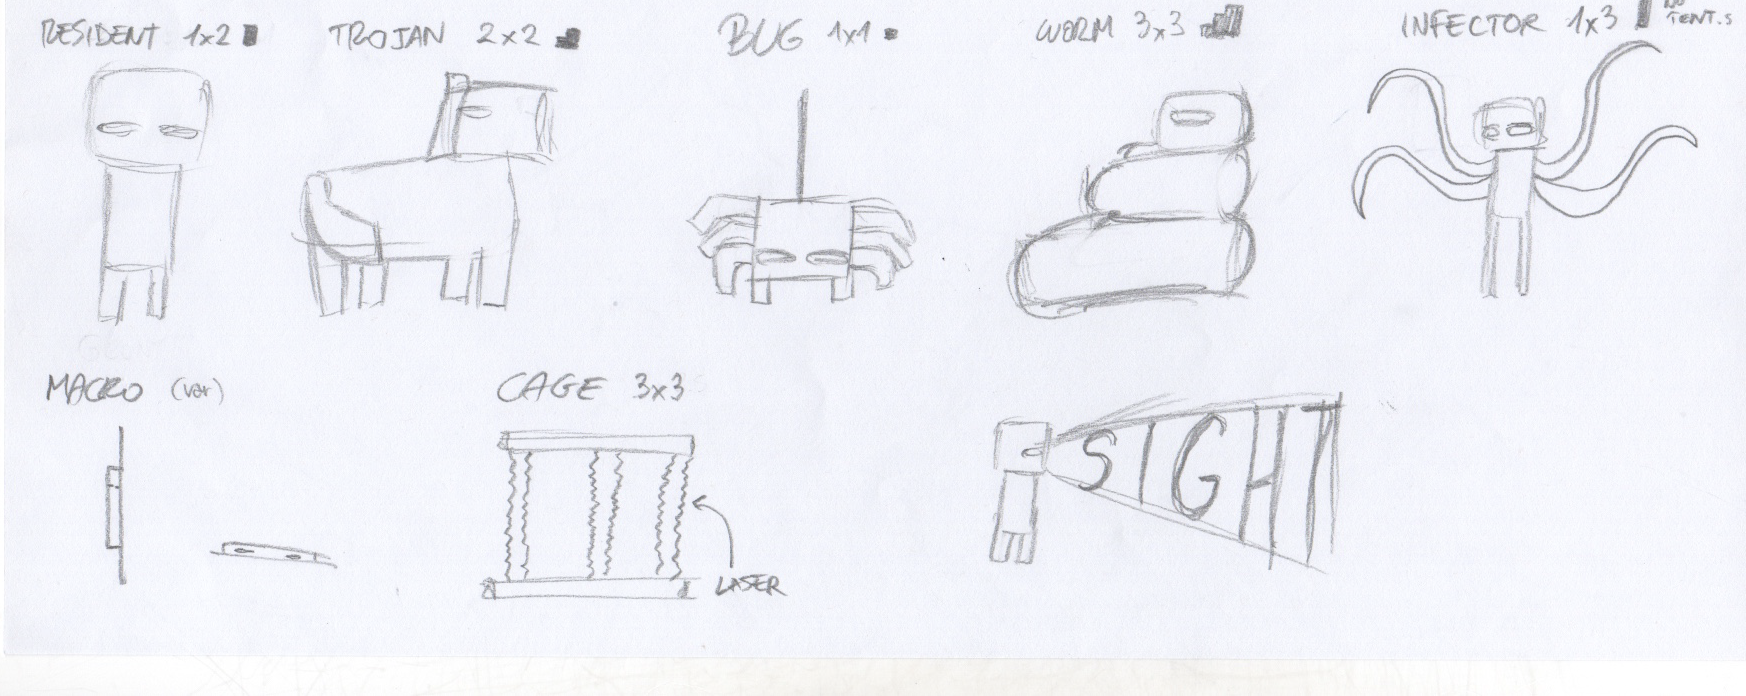
\includegraphics[width=0.5\textwidth]{images/Enemy}
\end{figure}
	\begin{figure}[H]
	\centering
	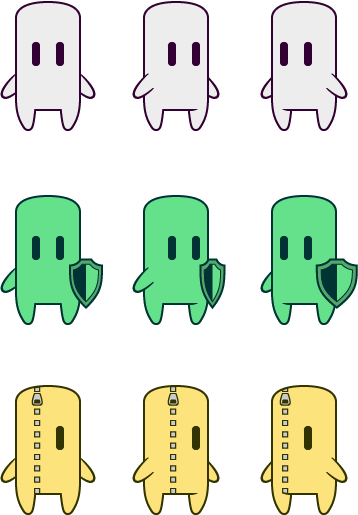
\includegraphics[width=0.3\textwidth]{images/Bits}
\end{figure}


\chapter{Sound Overview}
The soundtrack takes inspiration from electronic music, particularly on the “trance” and “chill” side, to make the player feel like they are in a virtual world.
The sound effects are mostly simple and monophonic, reminescent of old-school arcade games.\\


\end{document}
